\section[Wykład 8: 27-IV-2017 - Temat: Łańcuchy Markowa II]{Temat: Łańcuchy Markowa II}
\subsection{Wprowadzenie}
Metody MCMC (ang. \textit{Markov Chain Monte Carlo}), czyli metody Monte Carlo z wykorzystaniem łańcuchów Markowa wykorzystywanej między innymi przez Johna von Neumanna, Stanisława Ulama i Nicholasa Metropolisa w Projekcie Manhattan w celu za modelowania zbyt złożonych procesów matematycznych (na przykład obliczania całek).

\textbf{Procedura:} Wybierz punkt, {\color{green} poruszaj się losowo} tak, by {\color{red}szybko} punkt {\color{blue}zapomniał} o miejscu startu.


Ciekawa strona do wizualizacji łańcuchów Markowa: \url{http://setosa.io/ev/markov-chains/}
\subsection{Łańcuch Markowa}
\textbf{UWAGA!} w czasie tego kursu Łańcuch Markowa to Łańcuch o skończonej (rzeczywistej) liczbie stanów.

$\mathbb{P}=[\pi _{ij}]$, gdzie $\pi _{ij}$ to prawdopodobieństwo przejścia w w jednym kroku z $i$ do $j$.

$$\sum _{j\in S}\pi _{ij}=1,\ \pi _{ij}\geq 0$$
$\bar{p}(0)=(p_1(0),p_2(0),...,p_S(0)$ prawdopodobieństwo, że w momencie $0$ będziemy w stanie $i$\\
$p_i(t)$ prawdopodobieństwo w momencie $t$, że będziemy w stanie $i$\\
$$p_i(t+a)\sum _{j\in S}p_j(t)\pi _{ji}$$
$$\bar{p}(t+1)=\bar{p}(t)\mathbb{P}$$
$$\bar{p}(t)=\bar{p}(0)\mathtt{P}^t$$

\begin{definition}[Rozkład stacjonarny]\label{def:RozkladStacjonarny}
Rozkład prawdopodobieństwa $\bar{\pi}$ nazywamy stacjonarnym jeśli: $$\bar{\pi}=\bar{\pi}\mathbb{P}$$ 
$$\bar{\pi}=(\pi _1,\pi _2,..., \pi _n) : \sum _{i\in S}\pi _u =1, \pi _i \geq 0$$
\end{definition}

\begin{theorem}
Jeśli Łańcuch Markowa o skończonej liczbie stanów jest ergodyczny wtedy dla każdych dwóch stanów $i,j\in S$ i $$\lim _{t\rightarrow \infty }p_{ij}(t)=\pi _j$$ gdzie $$\bar{\pi}=(\pi _1,\pi _2,...,\pi _S)$$ jest wektorem stacjonarnym Łańcucha Markowa
\end{theorem}

$$\bar{p}(0)\mathbb{P}^t=\bar{p}(t)\underset{t\rightarrow \infty}{\rightarrow}\bar{\pi}$$

\begin{definition}[Nieprzywiedlność Łańcucha Markowa]\label{def:NieprzywiedlnoscLM}
Łańcuch Markowa jest \textbf{nieprzywiedlny} dla dla każdej pary stanów $i,j$ istnieje $t$ takie, że 
$$\pi _{ij}(t)>0$$ gdzie: $\pi _{ij}$ to prawdopodobieństwo przejścia ze sanu $i$ do $j$ w $t$ krokach.
\end{definition}

\subsection{Okres Łańcuchu Markowa}
\begin{figure}[H]
\centering
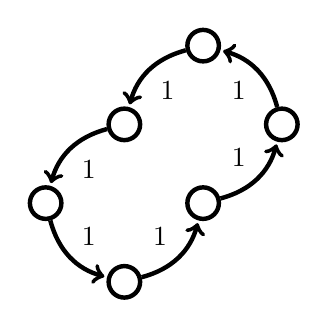
\begin{tikzpicture}[shorten >=1pt, auto, node distance=3cm, ultra thick,main node/.style={circle,draw,minimum size=.4cm,inner sep=0pt}]
\begin{scope}[every node/.style={font=\sffamily\large\bfseries}]
\node [main node](v1) at (0,0) {};
\node [main node](v2) at (1,-1) {};
\node [main node](v3) at (2,0) {};
\node [main node](v4) at (3,1) {};
\node [main node](v5) at (2,2) {};
\node [main node](v6) at (1,1) {};
\end{scope}
\path 
	(v1) edge [->,bend right] node {$1$} (v2)
    (v2) edge [->,bend right] node {$1$} (v3)
    (v3) edge [->,bend right] node {$1$} (v4)
    (v4) edge [->,bend right] node {$1$} (v5)
    (v5) edge [->,bend right] node {$1$} (v6)
    (v6) edge [->,bend right] node {$1$} (v1)
    ;
\end{tikzpicture}
\caption*{Łańcuch Markowa z okresem 6}
\end{figure}

\begin{definition}[Okres stanu Łańcucha Markowa]\label{def:OkresStanuLM}
Niech $i\in S$ będzie stanem Łańcucha Markowa.\\
Okresem stanu $i$ nazywamy liczbę:
$$\mathsf{okr}(i)=\underset{\text{największy wspólny podzielnik}}{\mathsf{nwp}}\{t: \pi _{ii}(t)>0\}$$
\end{definition}
\begin{definition}\label{def:OkresLM}
Okres Łańcuchu Markowa to
$$\mathsf{okr}(Ł)=\max _{i\in S} \mathsf{okr}(i)$$
Łańcuch Markowa nazywamy okresowy, gdy $\mathsf{okr}>1$
\end{definition}
\begin{fact*}\label{fac:OkresLM}
Jeśli Łańcuch Markowa jest nieprzywiedlny to wszystkie stany mają ten sam okres.
\end{fact*}
\textbf{UWAGA} Jeśli Łańcuch Markowa jest nieprzywiedlny i zawiera chociaż jedną pętle to jest nieokresowy,

\begin{definition}[Ergodyczność Łańcucha Markowa]\label{def:ergodycznoscLM}
Łańcuch Markowa jest ergodyczny, gdy jest nieprzywiedlny i nieokresowy.
\end{definition}

\begin{theorem}[Ergodyczność Łańcucha Markowa]\label{the:ergodycznoscLM2}%pobrane ze strony: http://smurf.mimuw.edu.pl/node/713
Dla skończonego nieredukowalnego i nieokresowego łańcucha Markowa $\mathbb{M}$ o zbiorze stanów $S$ istnieje wektor $\bar{\pi}$ którego elementy $\pi _a\,,a\in S$ takie, że:
\begin{enumerate}
\item $$\sum _{a\in S} \pi _a=1$$ oraz $0\leq \pi _a\geq 1$ dla wszystkich $a\in S$
\item $$\bar{\pi}\mathbb{M}=\bar{\pi}$$
\item dla każdego $a,b\in S$ zachodzi $$\lim _{n\rightarrow \infty} p_{a,b}(n)= \pi _b$$
\end{enumerate}
Pojawiający się w powyższym twierdzeniu wektor $\bar{\pi}$ nazywa się z reguły rozkładem stacjonarnym, co można łatwo zrozumieć patrząc na pierwsze dwa punkty tezy twierdzenia ergodycznego. Pierwszy z punktów mówi, że $\bar{\pi}$ jest rozkładem prawdopodobieństwa na zbiorze stanów $S$. Drugi punkt mówi, że jest on stacjonarny w następującym sensie: Jeśli $X_t$ ma rozkład $\bar{\pi}$, to $X_{t+1}$ także ma rozkład $\bar{\pi}$.

Najważniejszy jest oczywiście punkt trzeci, który mówi, że niezależnie od tego w jakim stanie łańcuch startuje, po odpowiednio długim czasie zbiegnie do rozkładu $\bar{\pi}$. Innymi słowy, niezależnie od rozkładu $X_0$, dla odpowiednio dużych $t$, zmienna $X_t$ będzie miała rozkład dowolnie bliski $\bar{\pi}$.
\end{theorem}


\begin{problem*}
Jak znaleźć rozkład stacjonarny Łańcuchy Markowa:
$$\bar{\pi}=\bar{\pi}\mathbb{P}$$
\end{problem*}

\begin{definition}[Odwracalność Łańcuchów Markowa]\label{def:OdwracalnoscLM}
Łańcuch Markowa jest odwracalny, gdy istnieje wektor $\bar{a}=(\bar{a_1}, ..., \bar{a_S})$ taki, że dla każdej pary $i,j$: $$a_i\pi _{ij}=a_j\pi _{ji}$$  wtedy wektor $\bar{\pi}=(\pi _1,...,\pi _S)$ taki, że $$\pi _i=\frac{a_i}{\sum _{s\in S}a_i}$$ jest wektorem stacjonarnym Łańcuchu Markowa.

\textbf{Uwaga!} wektor $\bar{a}$ jest niezerowy, posiada wartości nieujemne - niektóre jego współrzędne mogą być równe $0$
\end{definition}

\begin{example*}[Błądzenie po grafie]
Dany jest nieskierowany graf $G$. Z każdego wierzchołka $v$ z prawdopodobieństwem $\sfrac{1}{\deg (v)}$  udajemy się do ustalonego sąsiada $v$.

Czyli wybieramy losowo jednego z sąsiadów i idziemy do niego.
\begin{multicols}{2}
\begin{figure}[H]
\centering
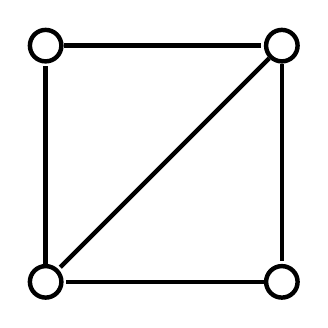
\begin{tikzpicture}[shorten >=1pt, auto, node distance=3cm, ultra thick,main node/.style={circle,draw,minimum size=.4cm,inner sep=0pt}]
\begin{scope}[every node/.style={font=\sffamily\large\bfseries}]
%\node (v0) at (-2,2) {START};
\node [main node](v1) at (0,0) {};
\node [main node](v2) at (3,0) {};
\node [main node](v3) at (3,-3) {};
\node [main node](v4) at (0,-3) {};
\end{scope}
\path 
%	(v0) edge [->] (v1)
	(v1) edge (v2)
    (v2) edge (v3)
    	 edge (v4)
    (v3) edge (v4)
    (v4) edge (v1)
    ;
\end{tikzpicture}
\end{figure}

\begin{figure}[H]
\centering
\begin{tikzpicture}[shorten >=1pt, auto, node distance=3cm, ultra thick,main node/.style={circle,draw,minimum size=.4cm,inner sep=0pt}]
\begin{scope}[every node/.style={font=\sffamily\large\bfseries}]
%\node (v0) at (-2,2) {START};
\node [main node](v1) at (0,0) {};
\node [main node](v2) at (4,0) {};
\node [main node](v3) at (4,-3) {};
\node [main node](v4) at (0,-3) {};
\end{scope}
\path 
%	(v0) edge [->] (v1)
	(v1) edge [->,bend left] node {$\sfrac{1}{2}$} (v2)
    	 edge [->] node {$\sfrac{1}{2}$} (v4)
    (v2) edge [->] node {$\sfrac{1}{3}$} (v1)
    	 edge [->,bend left] node {$\sfrac{1}{3}$} (v3)
         edge [->,bend left] node {$\sfrac{1}{3}$} (v4)
    (v3) edge [->] node {$\sfrac{1}{2}$} (v2)
    	 edge [->,bend left] node {$\sfrac{1}{2}$} (v4)
    (v4) edge [->,bend left] node {$\sfrac{1}{3}$} (v1)
    	 edge [->] node {$\sfrac{1}{3}$} (v2)
     	 edge [->] node {$\sfrac{1}{3}$} (v3)
    ;
\end{tikzpicture}
\end{figure}

$$\mathbb{P}=\begin{bmatrix}
0&\sfrac{1}{2}&0&\sfrac{1}{2}\\
\sfrac{1}{3}&0&\sfrac{1}{3}&\sfrac{1}{3}\\
\sfrac{1}{2}&0&0&\sfrac{1}{2}\\
\sfrac{1}{3}&\sfrac{1}{3}&\sfrac{1}{3}&0
\end{bmatrix}$$
\end{multicols}
\begin{align*}
&a_i\pi _{ij}=\frac{a_i}{\deg (i)}\\
&\text{Jeśli } a_i=\deg (i) \text{ to }\\
&\frac{\deg (i)}{\deg (i)}=a_i \pi_{ij}=a_j\pi _{ji}=\frac{\deg (j)}{\deg (j)}\\
&\pi _{i}=\frac{\deg (i)}{\sum \deg (i)}=\frac{\deg (i)}{2E}
\end{align*}
\begin{figure}[H]
\centering
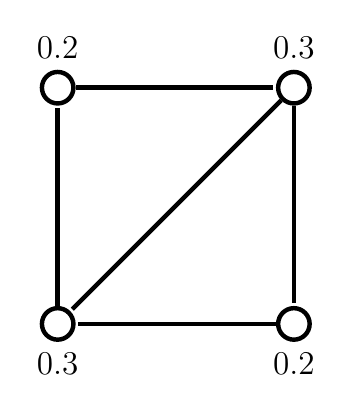
\begin{tikzpicture}[shorten >=1pt, auto, node distance=3cm, ultra thick,main node/.style={circle,draw,minimum size=.4cm,inner sep=0pt}]
\begin{scope}[every node/.style={font=\sffamily\large\bfseries}]
%\node (v0) at (-2,2) {START};
\node [main node,label=above:$0.2$](v1) at (0,0) {};
\node [main node,label=above:$0.3$](v2) at (3,0) {};
\node [main node,label=below:$0.2$](v3) at (3,-3) {};
\node [main node,label=below:$0.3$](v4) at (0,-3) {};
\end{scope}
\path 
%	(v0) edge [->] (v1)
	(v1) edge (v2)
    (v2) edge (v3)
    	 edge (v4)
    (v3) edge (v4)
    (v4) edge (v1)
    ;
\end{tikzpicture}
\end{figure}
\end{example*}

\textbf{Pytanie:} Kiedy Łańcuch Markowa odpowiadający błądzeniu po grafie $G$ jest ergodyczny?
\begin{itemize}
\item[] On jest nieprzywiedlny $\Leftrightarrow$ $G$ jest spójny
\item[] On jest nieokreślony $\Leftrightarrow$ $G$ nie jest dwudzielny
\end{itemize}
